% ------------------------------------------------------------------------ %
% !TEX encoding = UTF-8 Unicode
% !TEX TS-program = pdflatex
% !TEX root = ../Tesi.tex
% !TeX spellcheck = en_US
% ------------------------------------------------------------------------ %
%
% ------------------------------------------------------------------------ %
% 	PROPOSED SOLUTION
% ------------------------------------------------------------------------ %
%
\chapter{Proposed Solution}
%
\label{cap:proposedsolution}
%
% ------------------------------------------------------------------------ %
%
%
In this chapter the development of the solution will be reported step by step, with some use cases. The chapter starts with a list of solutions already developed, already on the market and he differences between them and my work. The remaining part is composed of two mains sections: the first explains the choice of the so called \textit{container}, the architecture, the type of file, etc. It lays the foundations and describes the limitations for the second part: the definition of the \textit{syntax}, or better the \textit{structure} of what is written inside the container. The two parts are closely related, therefore  their relation was taken into account when I made my choice. 
 \\
The real implementation of the valid solution is left for the next chapter.

\section{Already developed solutions}
A lot of companies have already tried to create a solution as "universal" as possible, but as their main aim is profit they are not really interested in creating a "real" universal solution. Their main goal is including more and more smart objects and making them compatible with their systems. The Web of Things for them is not an arrival point to reach, but rather an obstacle for increasing their profits. Companies are not innovating in the sense of creating a common framework that every vendor can use. They are trying only to enlarge their sphere of influence, not to be a real change in the world. This means companies aim to keep the IoT as final product to offer to users, doing it with some partnerships with the companies which produce smart devices. It is only a matter of time before some exclusive contracts will be signed: if some producer becomes a supplier for only one system, there is no gain for the community, a user has to choose which objects to buy depending on the system he has maybe already chosen and not depending on the specifications or the features of the device.\\
For instance we can analyze some products, such as \textit{Apple HomeKit}. Apple has built this groundbreaking application with the possibility to integrate devices to control a smart space, in particular a house. The idea is good, the application, in my opinion, is fantastic, but there are some limitations: the application can run only on iOS devices, and this constraint is somehow strict, as already explained in the first two point of the \ref{needforwot} section. Then, as explained here, the only devices that are compatible are the one which includes a particular protocol, always developed by Apple \cite{applehomekitprotocol}. It is called \textit{HomeKit Accessory Protocol (HAP)}, it is closed and vendors have to implement it inside the objects. This second requirement is stricter than what I have stated in \ref{problemdefinition} section, I only "impose" objects to have an HTTP connection and act as web servers: there is no simpler request to be on the web. Here it is different, HAP can work also on Bluetooth Low Energy (LE), but an upper layer is needed.
\begin{figure}[h]
	\centering
	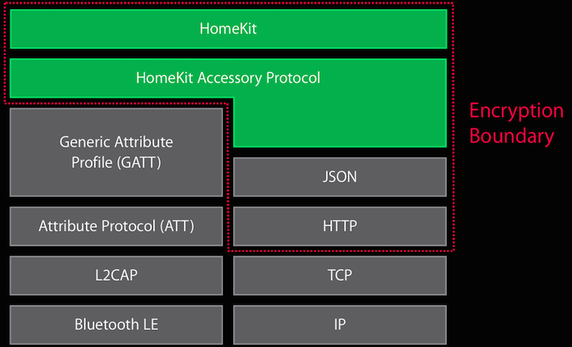
\includegraphics[width=1\textwidth]{hap}
	\caption{HomeKit Accessory Protocol (HAP)}
	\label{4.1: hap}
\end{figure}

I quoted this solution only to give the reader an idea of what is already existing, but many other systems are present on the market, Google has its system, called \textit{Google Brillo} that works similarly. Brillo is an Operative System (O.S.), obviously based on Android, which must be installed on the smart object. It "violates" my requirements about the liberty of a device concerning hot to reach the web and how to implement underlying layers. Also Microsoft has its solution, it enjoyed the \textit{Allseen Alliance}, an open solution that embraces all the levels of the protocol stack, using ad hoc developed layers. \\
All the solutions I have very briefly listed here are only some of the ones the market today offers. But they have a different purpose, they wants the devices mounting an operative system, a protocol, etc. This still remains in the situation explained in chapter \ref{cap:statoarte}, a war fought by different companies or alliances, leading the world to a myriad of different and incompatible solutions: it is more an attempt to enlarge each own IoT, respect than the creation of an open solution for a common widely resource like the web. Now it is the moment to start with my reflections about the given problem comparing the available paths to reach a solution.  


\section{Choice of the \textit{container}}
To better explain what I consider container it is important to understand the playground to my work. As said in the previous chapter, \ref{cap:probanalysis}, I am trying to fulfill the "horizontal" part of the connection in the stack, staying in layer 7, the application layer. Using already developed and operating tools, and respecting all the above listed constraints I am going to make the communication between WoT and IoT "HTTP ready" devices possible. I will now present alternatives to assure communications, choosing the one that better fits my requirements. The choice of the so called container is very important: it puts boundaries in the structure/syntax definition, so it is essential to understand pros and cons of each candidate. \\
I am searching for technologies that permit clients and servers to communicate, operating on the same network. The network is composed of three main actors: the user's client which is the web application opened, for instance, on a smartphone or a pc; the web server which it is the real application and it is on a machine which it behaves as a server for users and as a client for the smart objects; the objects, that have an end point on the HTTP protocol and behave as servers for the web server which asks information periodically. \\ 
What we need is a \textit{Web Service (WS)}. To understand what a WS is, there is the necessity to understand what we are doing and what we want to accomplish.

\subsection{Web Service (WS)} 
The web today is a sort of container of more than hyperlinks, it is a distributed application platform. If it is distributed data should be exchanged among nodes. What enables this exchange is the Web Service. A WS can be defined as a software component that permits data to flow among different applications (written in different programming languages) that runs on different operative systems, installed in different nodes of the network \cite{alonso2004web}. This mechanism does not put any limitation on the type of the application developed on the web and it is perfect. It does not affect the internal implementation of a web application, it is completely independent. A web service exposes some services, that can be "called" remotely to the other nodes of the network These services are often called \textit{APIs}, that stands for \textit{Application Programming Interfaces}, and they are particular functions that the developer of an application chooses to make reachable from others. It is possible to call the APIs through messages, more specifically W3C has standardized only one way to do it, through HTTP protocol. The WS has obviously some advantages and disadvantages that I will list. \\
Advantages:

\begin{itemize}

	\item Interoperability among different software applications that run on different hardware platforms is possible.
	
	\item Data format can be considered "textual", that is easy readable both for machines and humans.
	
	\item  Using HTTP for the transport of the message Web Services do not need any change in security rules of the firewalls of the nodes of the network.
	
	\item Web services are completely independent one from another, so they can be combined in a more complex and complete service offered to the user.
	
	\item There is no need to rewrite applications already existing to make them compatible to WS. They are completely independent also from modification done successively.  
	
\end{itemize}

Disadvantages:

\begin{itemize}

	\item Consolidated standards for critic applications, such as distributed transactions, do not yet exist.
	
	\item Some other alternative approaches for distributed computing can have better performances in some situations (Java RMI, CORBA, DCOM). They are briefly discussed later.
	
	\item They can "avoid" firewall controls and that can potentially be dangerous.
	
\end{itemize}

The main reasons of the wide adoption of Web Services are, as said, firstly, the "decoupling" between the service itself and the application behind it, without worries about modifying or rewrite one of the two sides, they are completely independent. Secondly, it uses HTTP over TCP on the 80 port, the one left (almost) always opened in each system so as to enable to surf the net  even company networks  that often have limitations for security reasons. \\
The Web Services have two main different implementations, \textit{SOAP} and \textit{REST}. These two approaches will be examined in the next subsections, now I will briefly focus on the alternative methods respect to these two. \\
The alternatives to Web Services are not taken seriously into account because they cannot be considered universal, as they are too closely related to a specific language or a set of languages. For example, \textit{Java RMI} stands for Remote Method Invocation and it enables to invoke a function on a remote object. Methods must be public and known by everyone. But it works only among Java sandboxes, so the application must be written in the Java language. It is a strict requirement for the whole web and it cannot be used in my work. \textit{CORBA (Common Object Request Broker Architecture)}, for instance, is another standard that can work with a set of different languages, which means not all the languages are accepted, but an intermediary is needed, called broker, which reads objects written in a special language that is IDL (Interface Description Language). And the translations between IDL and the specific languages are what makes CORBA compatible only with a defined set of programming languages. In any case this particular technique requires all the nodes of the networks to support it, an HTTP connection on 80 port is more and more simple.\\
These two examples, obviously, do not cover all the alternatives, but they are quoted to explain how the Web Services and their features are the most frequently used and effective solution. The next sections examine SOAP and REST and explain how and why I took my decision and reached my solution.\\

\subsection{SOAP protocol} \label{soap}
\textit{SOAP (Simple Object Access Protocol)}, as the name says, is a protocol that permits to call remote procedures (procedures are methods). This is enabled by an exchange of SOAP messages. SOAP is a member of the \textit{Remote Procedural Call} protocols family. SOAP is a standalone protocol that must be embedded in other protocols in order to surf the network and reach the proper node. The \textit{W3C} has standardized only HTTP to be the protocol which embeds SOAP, even if it is possible to embed also in the STMP (Simple Mail Transfer Protocol) one. SOAP can be viewed as a protocol that stays on top of the HTTP one and uses it as transport to reach every part of the network. It is older than its "opponent" REST, it was originally created by Microsoft and then submitted to the Internet Engineering Task Force (IETF) where it was standardized \cite{soap}. \\
Once it is understood that the fact that SOAP uses (mainly, but it is my case so I consider it a "standard") HTTP as a transport layer, we have to analyze the content of the message SOAP sends and receives. SOAP messages are based on the XML language that will now briefly explained. \\
Starting from scratch, \textit{XML (eXtensible Markup Language)} is a  language of markup, it means it has a syntactic mechanism to define and control the meanings of what is written inside. It defines the format of file .xml that can contain information which is possible to exchange on the network. It is composed of a hierarchical structure of tags, which can contain information (called also \#PCDATA, "Parsed Character Data") or other tags, it also is considered extensible because it is possible to create custom tags of any type only declaring them. As a small example, I report the following XML file, describing a list of users which can be, for example, the export of the contacts on a smartphone. \\

\begin{lstinputlisting}[
		language=XML,
		morekeywords={ciao,users,user,name,surname,number,bye},
		caption={XML file example},
		label=lst:xml]
		{Codici/example.xml}
\end{lstinputlisting}

The first line is called prologue and it is only a declaration of the XML version used and the encoding UTF-8 to interpret data correctly. The root tag, which is unique, is "users", that is a list of "user", each user is composed of a name, a surname and a number. The tags are formed by <> with in between the name of the tag. In this case tags are balanced: a tag is opened, then there is the content and finally it is closed. Also the nesting of tags is respected: opening "user" and then "name" I have to close the last one opened so I close "name" and then "user". These three properties (prologue, root that must be unique, balanced tags), if present, define a Well Formed XML. Having a WF XML it is possible to add a \textit{DTD (Document Type Definition)} file that contains rules to write a particular type of XML. DTD is out of our way, so I will not explain it in details. The only important thing is that it contains rules for writing XML, defining which elements can have sons, and type of information contained (link, string, etc). Another more recent type for the definition of the structure of an XML file is the \textit{XML Schema}, called also \textit{XSD, XML Schema Definition}. It is properly an XML file that defines a XML file and it supports datatypes (while DTD does not), and more generally it supports more options for defining precisely all the fields of the XML. If an XML file is Well Formed and it follows a DTD or XSD specifications, the XML file is called Valid.\\
In particular, a SOAP message is composed of a root tag called "soap:Envelope" that has two sons: "soap:Header" and "soap:Body", similar to the HTML structure. The header is optional while the body is mandatory. The header contains meta-information regarding routing, security, user identity, transactions etc. Two particular fields are remarkable: "MustUnderstand" that must be put equal to 1 if we want to oblige the reader to parse and read the header, because it contains vital information, for instance how to decipher a message. "Actor" contains the address of the recipient, so the intermediate endpoints can avoid to read the header. The body contains information, called payload. The payload has to follow a schema defined with a XSD, in order to assure that the SOAP message is Valid. The structure of the SOAP message just described is completely independent from the underlying protocol, HTTP, STMP, etc. that is used for transport \cite{soapMessage}.

\begin{lstinputlisting}[
		language=XML,
    morekeywords={ciao,soap:Envelope,soap:Header,soap:Body,m:GetQuotation,m:QuotationsName,ns1:applicationName,ns1:networkCode,ns1:RequestHeader,bye},
		caption={SOAP message example},
		label=lst:soap]
		{Codici/soapRequest.xml}
\end{lstinputlisting}

\medskip

The above file contains an example of a SOAP message that requires the value of Apple quotations to another node in the network. It is possible to identify all the elements previously described. \\ 
But, how can it be possible to know the right syntax of a tag to put in the "soap:Body" to have back a precise element? The \textit{WSDL (Web Services Description Language)} describes how the Web Services work, WSDL can be seen as a public interface of a Web Service \cite{curbera2002unraveling}. The WDSL is an XML file separated by SOAP messages, that is a sort of "handbook" of how to use the Web Service. It is mainly composed of three sections: "what" can be used, which means the operations that is possible to call through the network; "how" it is possible to use the service: the type of the protocol to use, the type of both input and output messages and the bindings of the service; "where", the endpoint to which it is possible to require the service, it is an URI. The WSDL can be divided also in another way: logic and concrete sections. The logic part contains interfaces, operations and messages, while the second  defines transport, bindings and endpoints. The current version is the 2.0 released in 2007 and it is a standard for the W3C. In the next listing I will give a example of WSDL, it is only an simple example to provide the reader with a more concrete idea of what we are talking about.\\

\begin{lstinputlisting}[
		language=XML,
    morekeywords={ciao,definitions,message,part,input,output,soap:operation,soap:body,service,documentation,soap:address,port,portType,operation,binding,soap:binding,bye},
		caption={WSDL file example},
		label=lst:soap]
		{Codici/wsdl.xml}
\end{lstinputlisting}

\medskip

Giving a brief description of the WSDL file, the tag "message" contains the type of message that the service has both in input or output and "name" indicates the parameter of the message, the tag "portType" describes the full available operation, indicating also which is the input message of the service and which one is the output, these two tags together are we what have called "what" previously; the tag "binding" is the "how", it explains that the service is reachable with the SOAP protocol and specifies the body of the message; finally, the tag "service" indicates the endpoint to which is possible to request the service, it is the "where" section previously defined. \\
Back to SOAP, one thing remains to be said, it is highly extensible, in particular some modules can be added: the term \textit{WS-*} stands for Web Services, but the * indicates all the possible ones. An extension is a variation of "something" in the SOAP message to emphasize a specific feature. Lots of extensions exist: for instance, WS-Security (WSS) is one concerning security, it can be used for some particular application where an identification or even authentication is required, it becomes less useful for open application. It guarantees, for example, end-to-end security, identification tokens and many other features.   

\subsection{REST paradigm}
The SOAP protocol and all its "environment" are only the first alternative we have to enable Web Services. The second one is the architecture called \textit{REST (REpresentational State Transfer)}, it was conceived for systems of distributed hypertext, as the web is today \cite{fielding2000representational}. In fact the World Wide Web is the most successful field in which the REST paradigm is used, but not the only one. The first thing to specify is that while SOAP is a particular, well defined protocol, standardized with a specific set of rules to follow, REST instead is a set of guidelines, a paradigm as just said, for the realization of a "system architecture". The word REST, indicating a "way to do things", can be considered the opponent of the term Remote Procedure Call (RPC), that indicates the procedure previously described, rather than SOAP, but, a unique implementation of a RESTful device does not exist I am putting them on the same level here. Note that a service implementing the REST paradigm is called \textit{RESTful service}.\\
Basing our analysis only on the web it is possible to state that REST is based on the concept of transmitting information over HTTP without the use of an upper optional layer such as CORBA, SOAP or the cookies used in websites nowadays. REST paradigm is based on principles that the web today knows very well, but they are somehow reinvented to be part of a Web Service. Firstly we have to define what can be considered \textit{resource} for the web:

\begin{itemize}
	\item A resource is every web element that had an elaboration. It is possible to compare a resource to an instance of an object in the Object Oriented programming paradigm.
	
	\item A resource can contain the state of an application or the functions it provides.
	
	\item A resource is uniquely identifiable by a string called \textit{URI (Universal Resource Identifier)}, a URI can be seen as the link to put together more than one resource.	
\end{itemize}

Having defined what a web resource is, the REST paradigm follows some other principles to exchange information among nodes of the network. The resource is what permits the sharing, but even the exchange process has to follow some guidelines respect to REST principles. The resources are shared as a common interface to allow the transfer of states among resources. The main features of the transfer are:

\begin{itemize}
	\item a fixed set of well known operations.
	
	\item a fixed set of contents, maybe with a particular request code.
	
	\item a protocol, that itself has to be:
		\begin{itemize}
		
			\item client-server: the division is strong, every part has its role, for instance, the client has no worries about saving information while the server has no worries about the graphical interface. If the interface that links them remains the same it is possible to modify them separately.
			
			\item uniform interface: client and server need a homogeneous interface. The two parts can evolve separately from the interface.
			
			\item stateless: no context is saved in the server, every request coming from the client has all the information needed to serve it.
			
			\item cacheable: the client can cache answers, but they have to declare if they are cacheable or not in order to prevent the use of wrong and invalid old answers. On the other hand the cache can reduce the number of client-server communications, increasing performances. 
			
			\item layered system: there is no only one server, it is possible to introduce some middleware servers to improve scalability with load-balancing or distributed caches. In addition the multi-layer models enables to introduce more secure mechanisms, isolating the information from external attacks.
			
			\item code on demand (optional): servers can send executable code that the client will interpret or compile, such as JavaScript. 
			
		\end{itemize}
		
\end{itemize}

Now that the main features have been presented, I will briefly informally describe the full procedure of a RESTful service.
Knowing a source of information (the resource), through the URI, the client can make a request and the server can "listen" what is requested. This communication happens through a standard interface (for example HTTP protocol). In this way representations of the resource  can be exchanged: receiving the request the server can answer in multiple ways, without knowing the "past story" between the two parts. There can also be the intermediation of middleware components, proxies, firewalls, etc, this does not affect the final result. The only thing the client needs to know is "what" is returned by the server: the format of the file is very important, the client needs to be able to process it once received. Typically the format is a HTML, XML or JSON file containing the information but answers, for instance, may also  be given with a picture. \\
The use of HTTP makes requesting and interacting with the information required very simple: this protocol provides a set of primitives, functions implemented directly inside that can be used by everyone. REST uses four of these verbs: \textit{GET, POST, PUT} and \textit{DELETE}. For example, the state of service can be obtained performing a HTTP GET to the URI, while in a not RESTful service we can custom methods, with arbitrary names depending on the implementation. In addition, one of the most important things is that HTTP verbs are 1:1 mapping to \textit{CRUD} operations. CRUDs are the fundamental operations that a user can execute on a resource. (More generally four actions must be implemented in a RESTful application, in a relational database and in a document management application to consider them "complete").

\begin{table}[h]
%
\caption{Mapping between CRUD operations and HTTP 1.1 verbs.}
%
\label{tab:crud}
%
\centering
%
\begin{tabular}{lll}
%
\toprule
%
\textbf{HTTP Verb} & \textbf{CRUD Operation} & \textbf{Description}\\
%
\midrule
%
POST & Create	& Create a new resource \\
GET & Read	& Obtain an existing resource \\
PUT & Update	& Update or change the status of a resource \\
DELETE & Delete	& Delete a resource \\
%
\bottomrule
%
\end{tabular}
%
\end{table}

In this way the HTTP protocol can cover all the possible actions a user can perform on a resource. This is one of the strengths of the REST paradigm. \\
At this point we have described what REST means, how it works and how it covers the operations needed to handle a resource. Now we will focus on the representation of this last component: what comes to the client is never the resource itself, it is always a representation. As said before there are no constraints on the type of file that is going to represent the resource on the client side, anyway it is better to uniform or, better, circumscribe the number and types of file that a RESTful service outputs. If the servers offers more than one representation it is possible for the client to choose one, indicating it in the "Accept" field of the request message. For example, a browser, when we go to a particular website, is doing an HTTP GET with the predefined "Accept" field equal to "HTML". In this case we have a Web UI, with all the graphical elements, pointing to the same page, changing the "Accept" to "JSON" we have a Web API. Following the REST principle, we can construct different architectures using the same URI, the same resource but changing its representation.\\
In the following pictures I am going to quickly describe HTTP messages, requests and responses, to have a full comparison with SOAP messages. Then a description of each sector of the message is provided.

\begin{figure}[h]
\centering
\subfloat[][HTTP Request\label{fig:pantoinpresa-simm}]
   {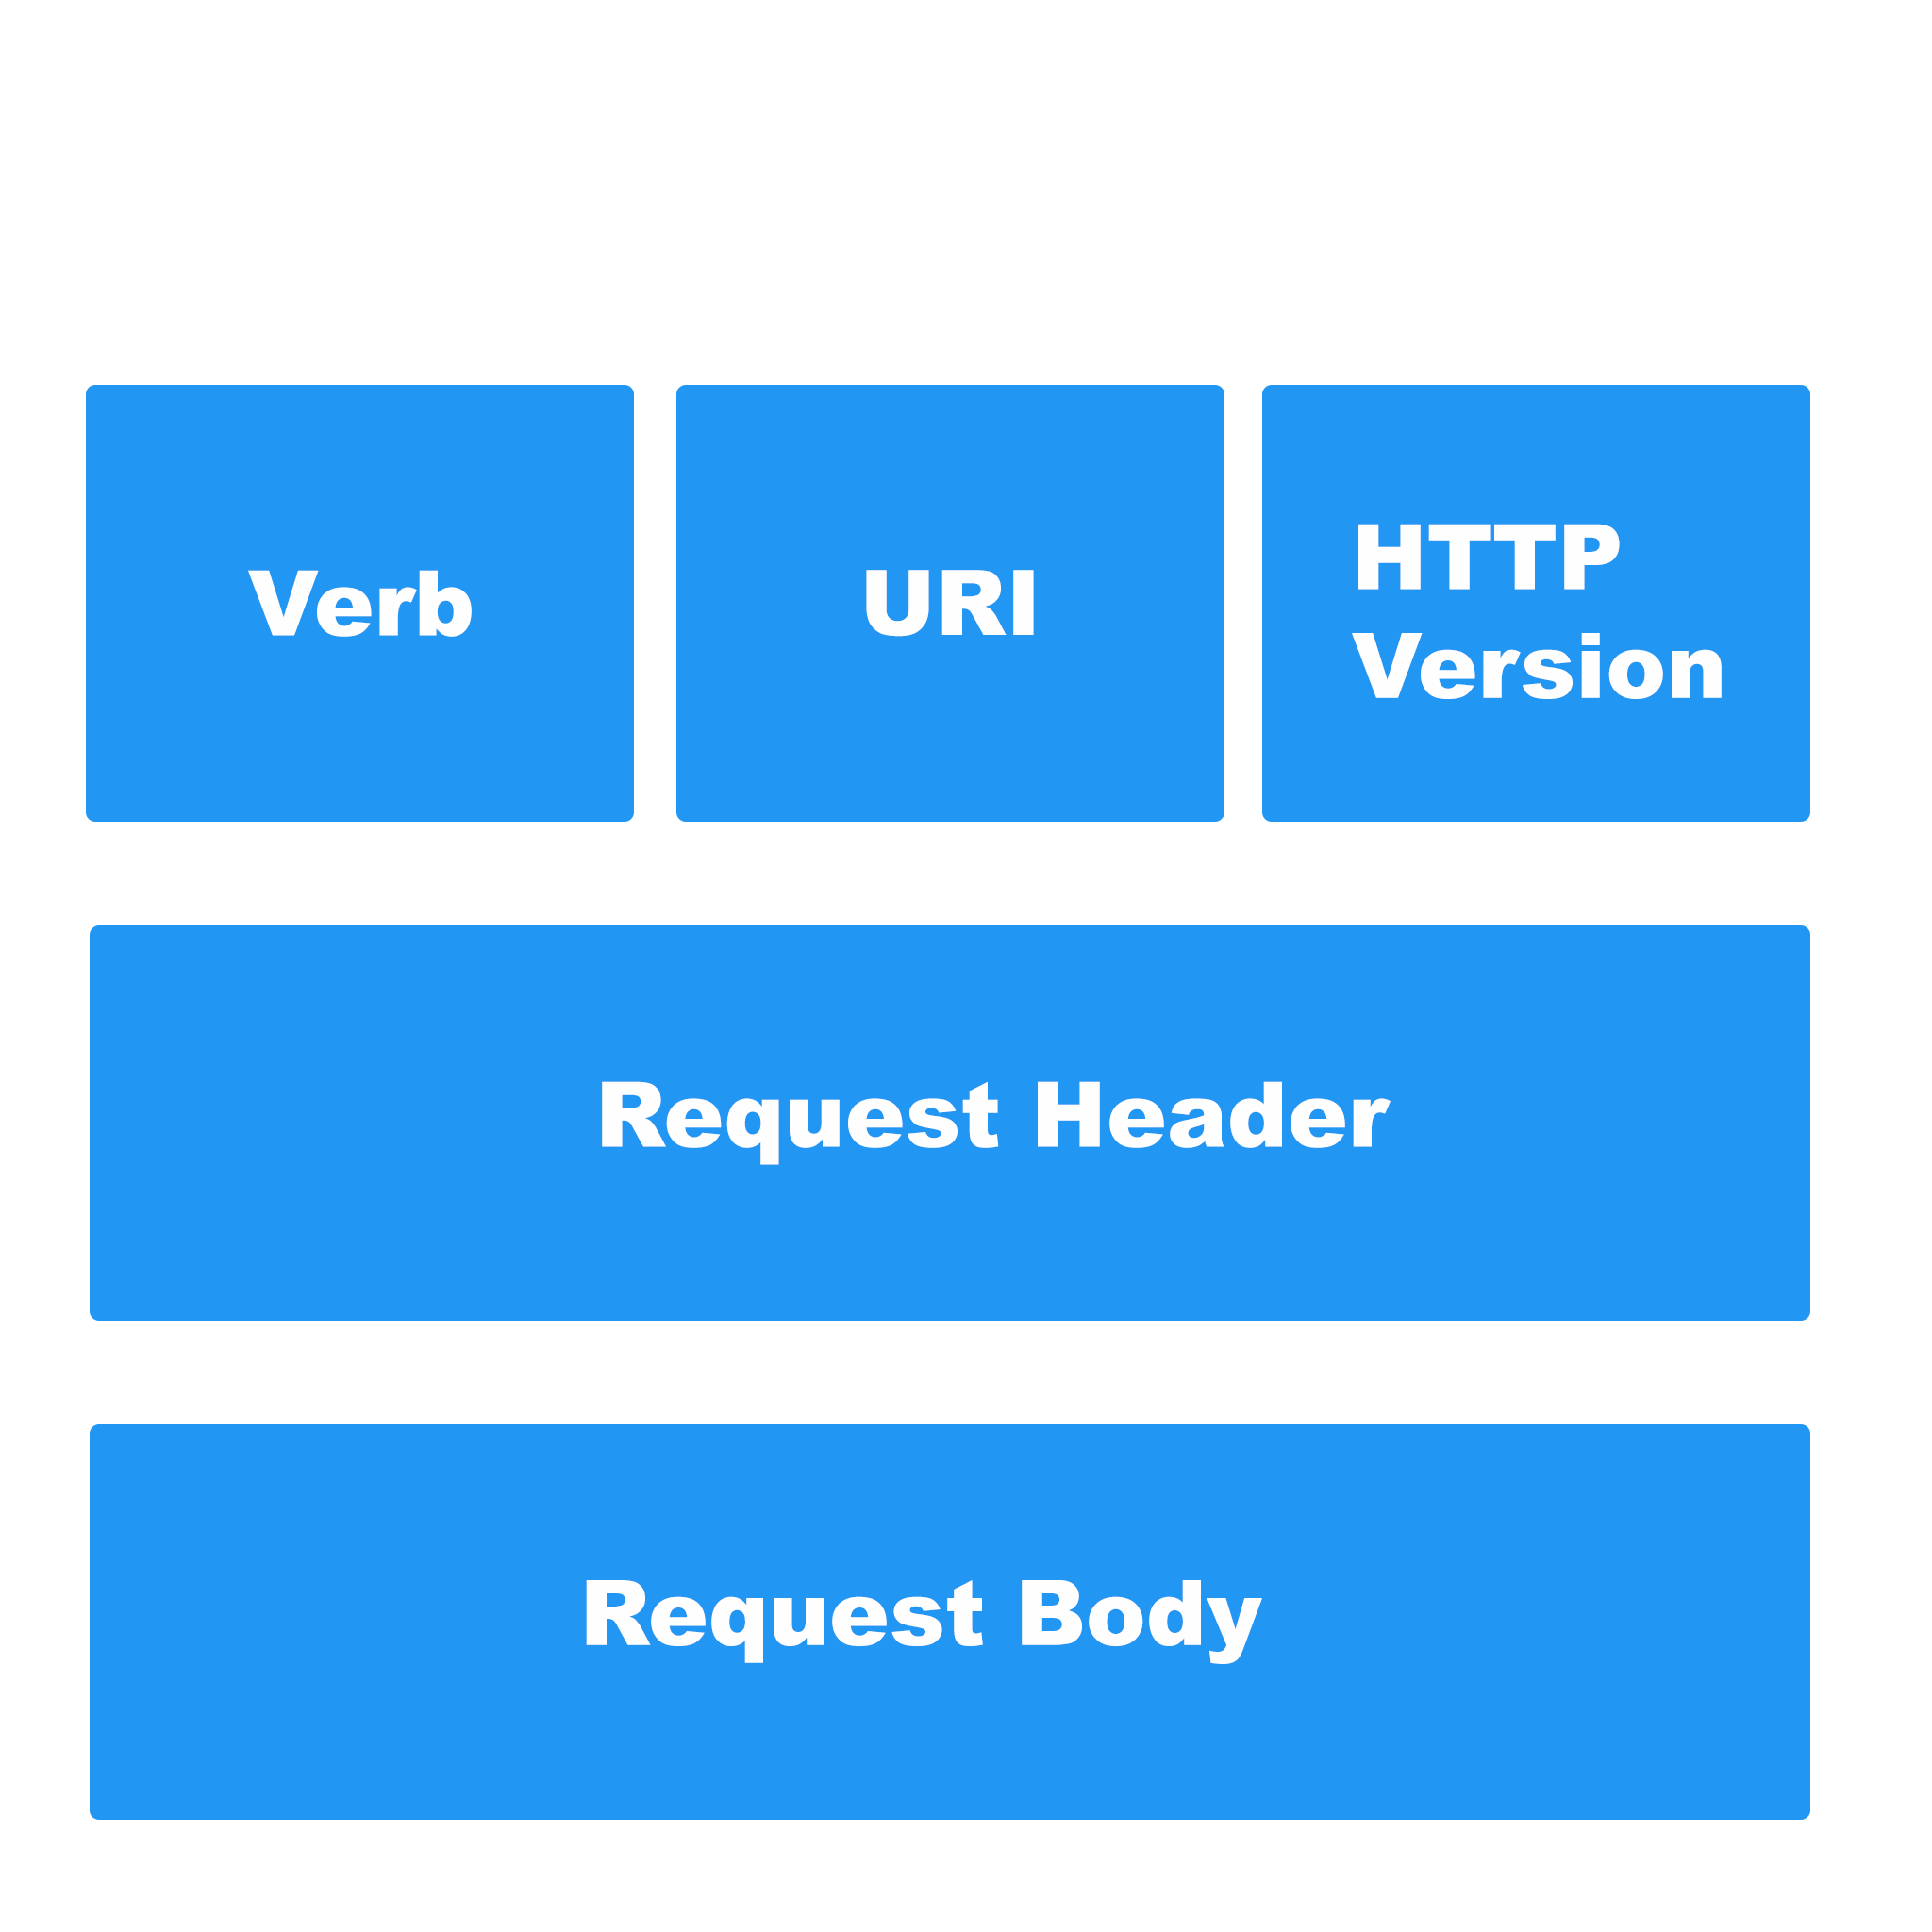
\includegraphics[width=.48\textwidth]{httpRequest}}\quad
\subfloat[][HTTP Response\label{fig:pantoinpresa-asimm}]
   {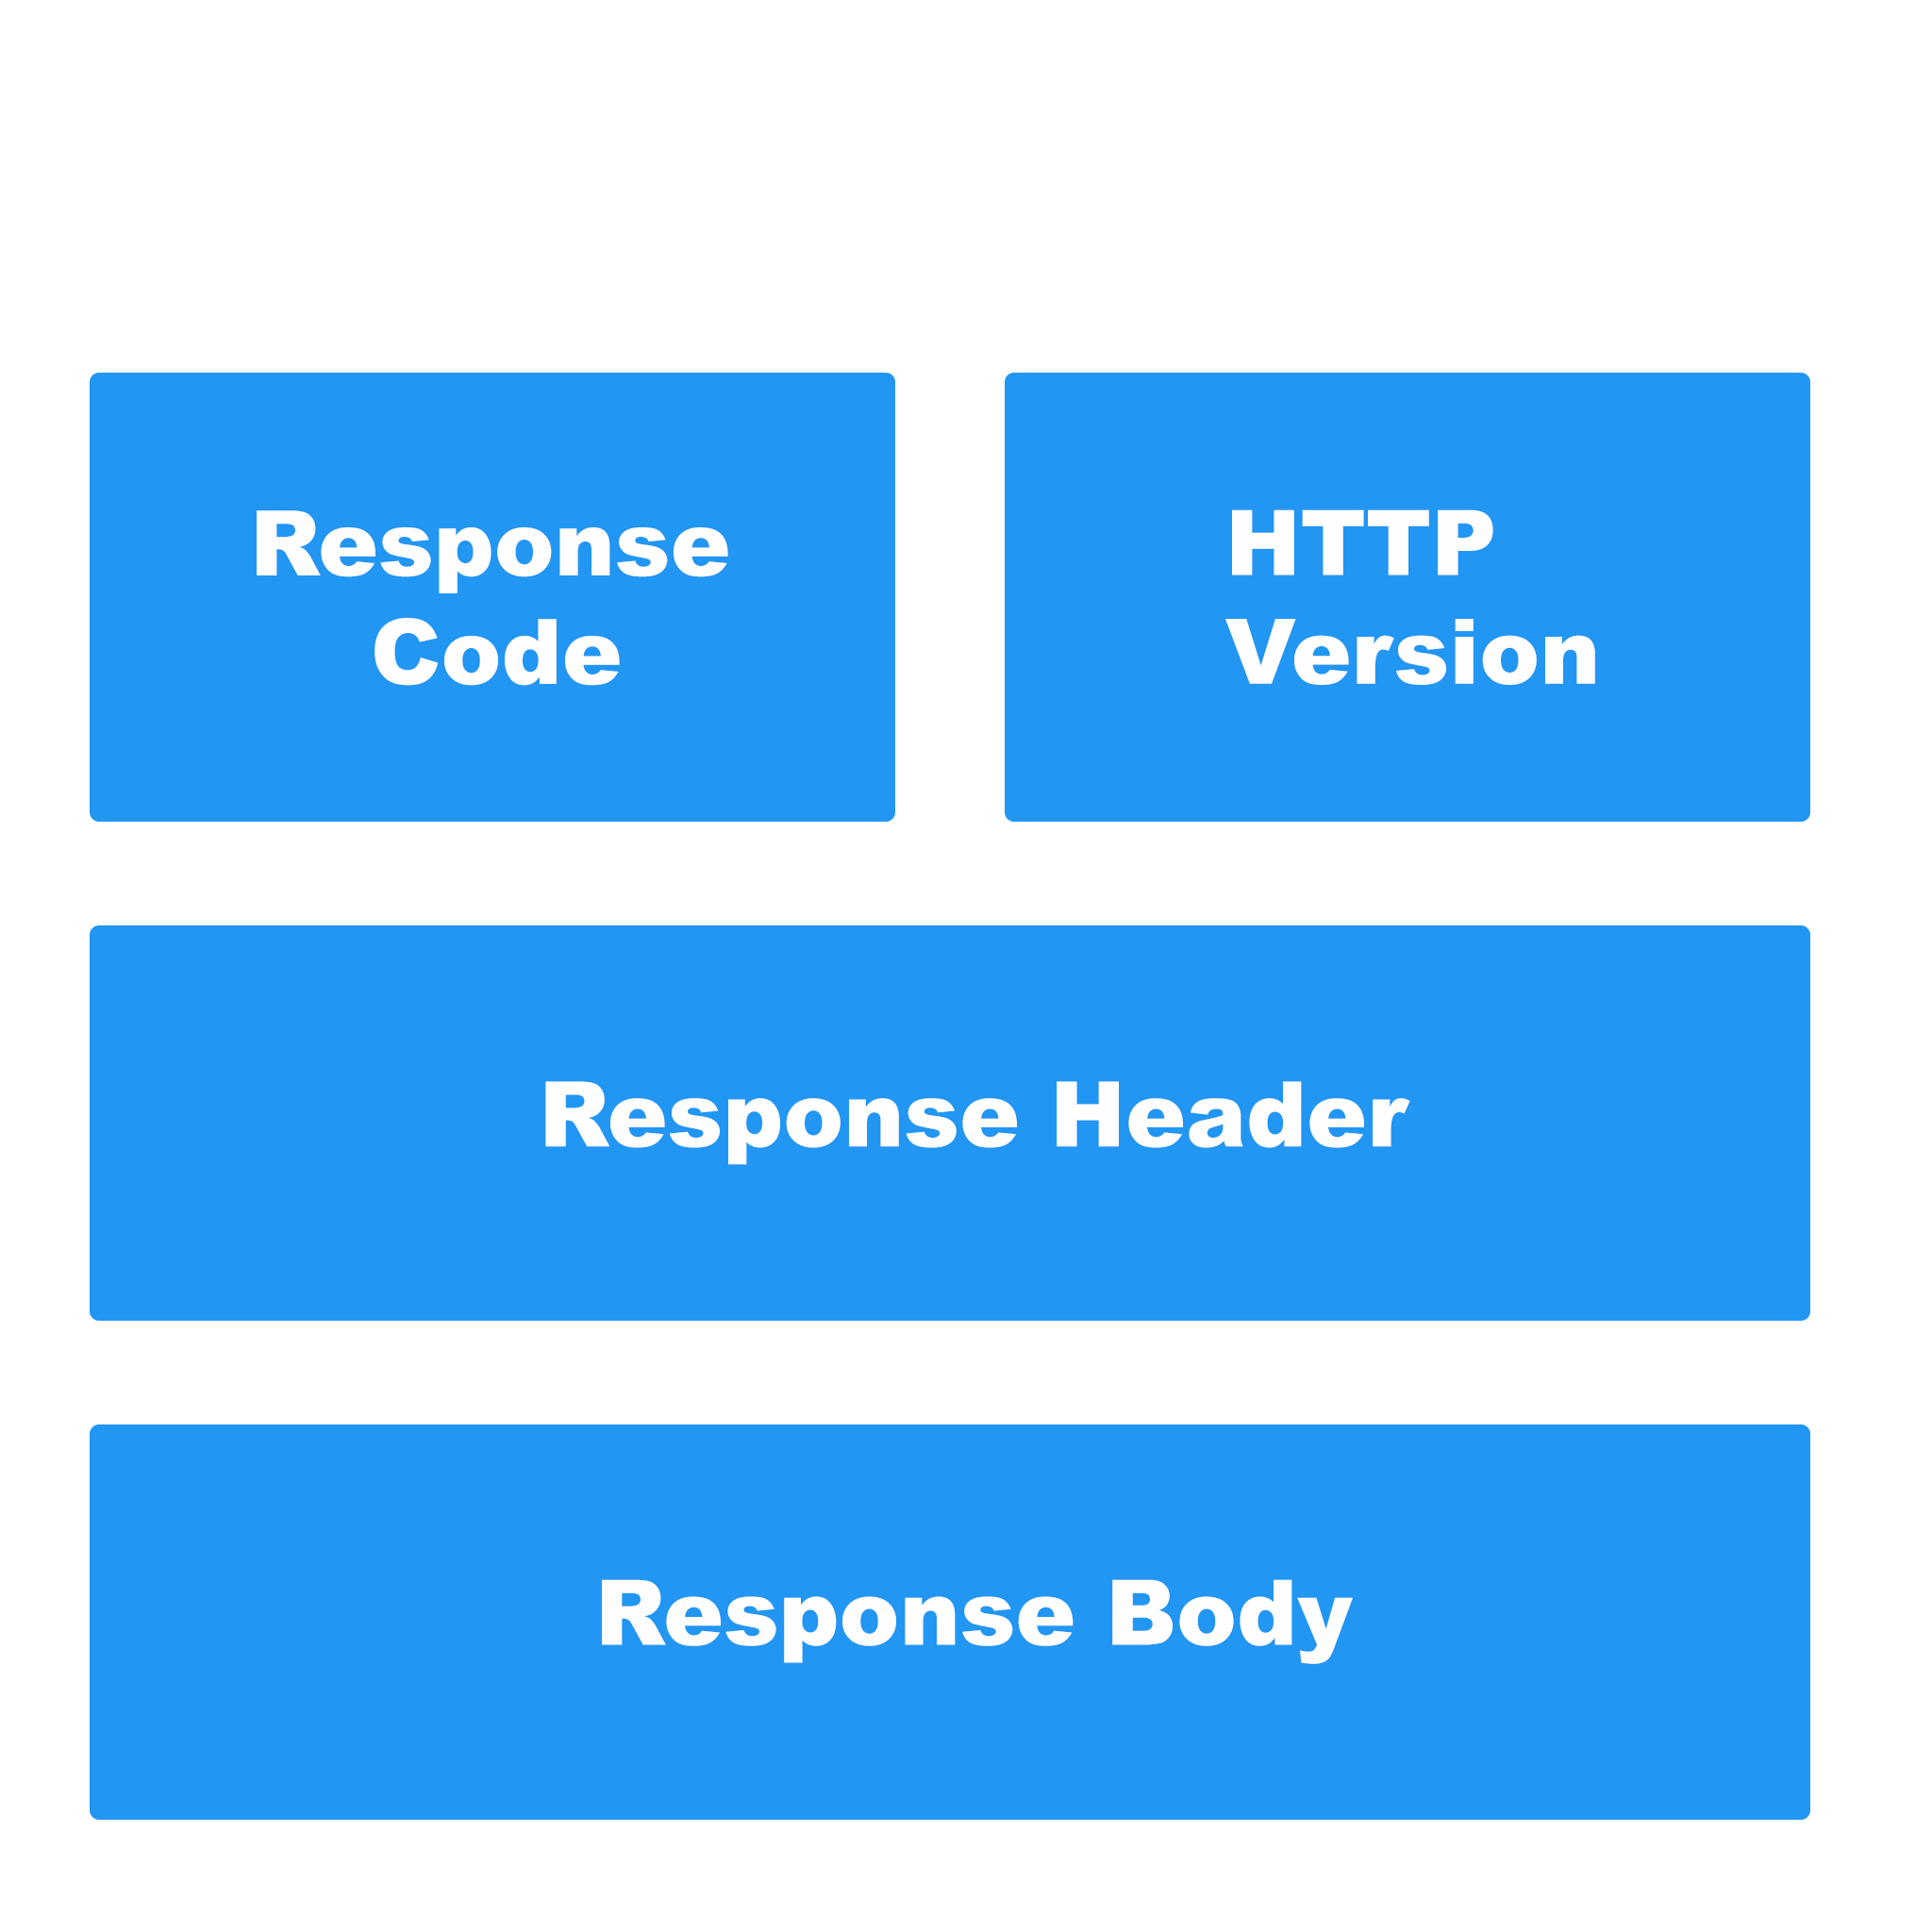
\includegraphics[width=.48\textwidth]{httpResponse}}
\caption{HTTP Messages}
\label{4.2:httpmessages}
\end{figure}

The HTTP Request message is composed of main 5 sectors:
\begin{itemize}

	\item Verb- Indicate HTTP methods such as GET, POST, DELETE, PUT etc.

	\item URI- Uniform Resource Identifier (URI) to identify the resource on server

	\item HTTP Version- Indicate HTTP version, for example HTTP v1.1 .

	\item Request Header- Contains metadata for the HTTP Request message as key-value pairs. For example, client ( or browser) type, format supported by client, format of message body, cache settings etc.

	\item Request Body- Message content or Resource representation	
	
\end{itemize}

An HTTP Response message has four major parts:
\begin{itemize}	

	\item Status/Response Code- Indicate Server status for the requested resource. For example 404 means resource not found and 200 means response is ok.
	
	\item HTTP Version- Indicate HTTP version, for example HTTP v1.1 .

	\item Response Header- Contains metadata for the HTTP Response message as key-value pairs. For example, content length, content type, response date, server type etc.
	
	\item Response Body- Response message content or Resource representation.

\end{itemize}

The stateless communication is done to maintain scalability inside the server, an open connection or session is a waste of energy and memory space: if too many requests come together the server can crash, it is the base of a DDOS attack for not RESTful services.


\subsection{Comparison and choice}
We have discussed in an appropriate way the two main candidates for the given problem. Here I would like to list pros and cons of both solutions and then choose which container to use, in particular the pros of a system can be considered the lacking items of the other, in the sense that if one feature is on a list it means that it is exclusive of that architecture:
\begin{itemize}
\item REST is generally easier to use and is more flexible:
	\begin{itemize}

		\item No expensive tools require to interact with the Web service 
		
		\item Smaller learning curve

		\item Efficient (SOAP uses XML for all messages, REST can use smaller message formats)
	
		\item Fast (no extensive processing required)
	
		\item Closer to other Web technologies in design philosophy
	
	\end{itemize}

\item SOAP is definitely the heavyweight choice for Web service access:
	\begin{itemize}

		\item Language, platform, and transport independent (REST requires use of HTTP)
	
		\item Works well in distributed enterprise environments (REST assumes direct point-to-point communication)
	
		\item Standardized
	
		\item Provides significant pre-build extensibility in the form of the WS* standards
	
		\item Built-in error handling
	
		\item Automation when used with certain language products
	
	\end{itemize}	
	
\end{itemize}

Taking a look at the points listed above, I would remark how the pros of the REST paradigm match some of the requirements already listed in \ref{problemconstraints}. Efficient and fast were two of the main characteristics needed by our system. Then the fact no expensive tools are needed is another important point, developing a sort of framework for third-party applications. Another advantage of REST is being "language independent". In addition it can be chosen only as "container", leaving the choice of the type of file free, even if we stated that it is better to limit the formats of file sent on the web. As far as SOAP advantages are concerned, it is important to underline how the fact it is independent from HTTP (while REST is dependent) is not a problem because we are talking about the Web of Things, we are supposing to put everything on the web, and the HTTP protocol is one of web's fundamental parts. The only point that can tilt in SOAP direction is the fact that SOAP is standardized while REST is not, it is a set of guidelines, not a well defined structure \cite{pautasso2008restful}.\\
As the reader can guess, the choice for my system is the REST paradigm. Despite the fact it is not standardized, REST provides a set of easier "rules" to build and develop a framework easily. The not-standardized part is what I am going to define in the next section of my thesis. Basing my own architecture on the HTTP messages and REST paradigm, the choice of the file surfing the web is still undecided, and the universal syntax I propose is still to be created.


\section{Structure definition}
This section is intended to define the format of file of my REST solution, and then the syntax inside it. As previously said, every format of file can be embedded into HTTP body and sent on the internet but it is a good habit to limit the number of circulating formats. In particular we can identify what is needed for our problem, restricting the choice. \\
We need to send to an application, a control center, the description of a smart space, in order to permit the user to control everything. The heterogenous elements are collected with a sort of "discovery", while in my application some "plugs" for particular chosen protocols are created. \\

\subsection{Available alternatives}
So we have to send descriptions of objects, the descriptions are composed of strings and numbers. It is possible to identify three main formats to send this type of information: HTML, XML and JSON. 
\begin{itemize}

	\item \textit{HTML:} the first format is the classical building block of a web page, it is a language that contains graphical elements, it is created for the web and it is in line with our intent but it is intended for humans, in particular for M2H communications, the final recipient is a human being. This doe not match our requirements: we need, as explained in \ref{problemconstraints}, a easy readable language but principally for a machine, my work needs to be a framework, something that links objects of the Internet of Things and the final UI the user will see. For this reason I am going to eliminate from the list of eligible candidates the HTML opportunity. It is the developer that will use my work as input to use, almost surely, HTML as language to speak to people.
	
	\item \textit{XML:} this language is approximately suitable for my purpose, it has all the credentials to be the choice, but it can be considered so much verbose and heavyweight compared to JSON. Anyway I am not going to deepen XML because it is already been done in \ref{soap}, explaining what kind of language SOAP uses.
	
	\item \textit{JSON:} JSON stays for \textit{JavaScript Object Notation}. It is a language created for data exchange in a client-server architecture. It is the choice I have made, and in the following subsection there is a full description what it is, how it works and above all how it can fit perfectly my requirements for the thesis.

\end{itemize}

I chose JSON for its lightweight, simplicity in writing and reading and also because there is a proposal of W3C to elect JSON to the official language for IoT and WoT. Firstly, I will discuss all the features of JSON, then I will do the same thing for one of its extensions \textit{JSON-LD}, I will present the W3C proposal and finally my solution, remarking what changes respect to others already developed.

\subsection{JSON} \label{json}
JSON (JavaScript Object Notation) is a lightweight data-interchange format. It is easy for humans to read and write. It is easy for machines to parse and generate. It is based on a subset of the JavaScript Programming Language, standardized in December 1999. JSON is a text format that is completely language independent but uses conventions that are familiar to programmers of the C-family of languages. These properties make JSON an ideal data-interchange language. \cite{jsondef} \\
It is based mainly on two types of structures: 

\begin{itemize}

	\item \textit{Key/Value pair set:} it can be considered an object of an Object Oriented programming language. It is "contained" by a left ({) and right (}) curly brace, each element of the set is separated from others with a coma (,) and it is composed by a \textit{key}, that is a string, followed by semicolon (:), followed by the \textit{value}.
	
	\item \textit{Collection of elements:} it can be considered an array, but it covers only \textit{values}, in the sense that in an object, we can define a key, write the semicolon but the values associated to the key are multiple, so they are put in an array. Syntactically they are composed of a left square bracket ([), values separated by commas (,) and after the last value there is a right square bracket (]).

\end{itemize}

It is important to know what can be assigned to the \textit{value} field. A \textit{value} can be an array, as just said, a string, a number, a \textit{boolean value} (true or false), \textit{null} or another object, constructed as above. This means that nested structures are allowed in JSON format. String are wrapped in double quotes (""), using backslash escapes, empty strings are allowed. The concept of the string here is the same of Java, for instance. \\
While XML can be considered a markup language, JSON is more a format created for exchange of data. In both language there is no concept of binary data, so the developer has to convert data from the binary format while writing (eg. an integer into a "textual form").\\
As for XML, a "schema" exists: for XML is called XSD, while here simply \textit{JSON data schema}. It can be used to validate JSON data. As in XSD, the same serialization/deserialization tools can be used both for the schema and data. The schema is self-describing. Anyway it is not a standard like XSD, but only an "Internet Draft (I-D)" proposed by IETF (Internet Engineering eTask Force), in order to become standardized.\\
In the above picture I am going to report in graphical way what has just been described, the syntactic rules to compose a JSON document, in order to give the reader a easier way to understand the format.\\

\begin{figure}[h]
	\centering
	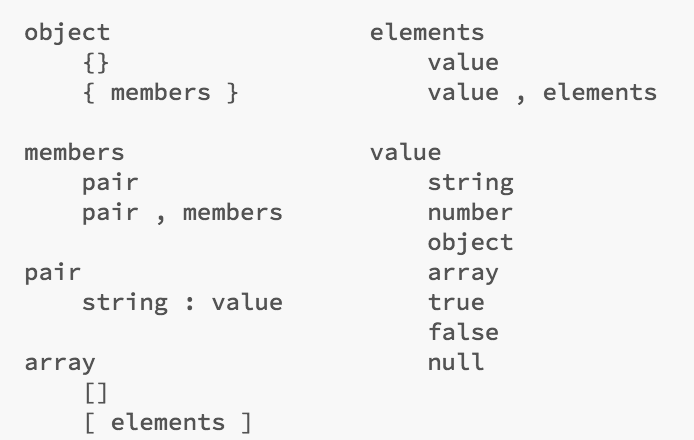
\includegraphics[width=1\textwidth]{json}
	\caption{JSON syntax rules}
	\label{4.3:json}
\end{figure}

JSON format is both \textit{M2M} and \textit{M2H/H2M} constraints compliant, and also \textit{easy readable} (and writable). Having these properties we can also state is \textit{fast}: both machines and humans are quick in doing actions on it. It is also \textit{lightweight}, in particular respect to XML, being less verbose and less depending on open-closed tags. Finally, as it is possible to see from the above picture it is \textit{modular} and \textit{extensible} with the possibility to nest levels. 

\subsection{JSON-LD}
\textit{JSON-LD} stays for \textit{JavaScript Object Notation for Linked Data} and it is intended to be an extension, an evolution to the JSON: it brings the web to a semantic level. To understand what is the \textit{Semantic Web}, I have to firstly explain what are \textit{Linked Data}.

\paragraph{Linked Data and Semantic Web} The internet is seen as a network composed of nodes that are "bare metal" objects: computers and servers principally, or smart objects. The web, in the same way, is a network, but it is composed of nodes that are websites or web applications. These nodes are linked, with URIs, as widely explained. While the humans can understand what a link stands for, based on where is put in a page or which keyword is put near it. The machines cannot have this idea, for them a link is simply a reference to another "portion of the web", another web page to download. To make the machines understand what a link is and what represent in that particular context, there is the need to construct linked data. Linked data are simply a way to make the machines conscious of what they are facing: in this way also computers can have a global vision of the web as a graph, almost connected, understanding the relations existing among different pages or applications. If, for example, we define on the web the concept of human being and the relation "marriedTo", the computer can know that the the object of the relation is another human being, so it can expect some type of data and it can raise an error if, for instance, the received type is a cat. This understanding can lead, for example, a computer to be more and more precise and capable of answering complex queries like "Who is Thomas father?": knowing the relation "father", the machine has only to follow the link provided to get and show the answer. A semantic cognition is what modern search engines are trying to reach.\\ 
\textit{Meta-data} is what permits the recognition, like a index for a library: there you can find all the useful information to catalogue the real information, the books. Here is the same, meta data, specified and filled in the HTML page are what permits the computer to know the relations existing among what it has already downloaded and what it can reach from there. \\
If the web, a complicated graph, has the possibility to be understood by a machine, we are talking about semantic web. A web with a with a consciousness of itself. \cite{bizer2009linked} \\
I will now report a figure, explaining graphically the concept of semantic web, using \textit{RFDa (Resource Description Framework in Attributes)} syntax. RFDa is a W3C Recommendation that adds a set of attribute-level extensions to HTML, XHTML and various XML-based document types for embedding rich metadata within Web documents. Anyway RFDa is beyond our purpose so it is not explained in depth.  

\begin{figure}[h]
	\centering
	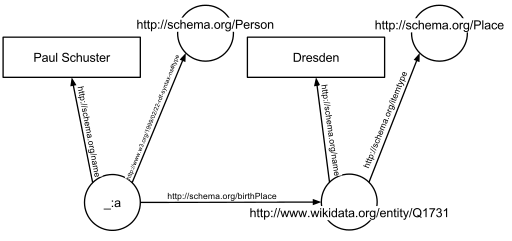
\includegraphics[width=1\textwidth]{semanticWeb}
	\caption{An example of semantic web}
	\label{4.4:semanticWeb}
\end{figure}

The node here called "\_:a" is a node of type "person", a URI  (\url{http://schema.org/Person}) defines what a "person" is. The "person" here has two different properties: "name" and "birthPlace". The "name" property is a string ("Paul Schuster"), a "terminal" (because it is not expanded, identified by a rectangular shape) property of the category "person". The property "birthPlace", on the other hand, is not a "terminal one", identified by a circle shape. It is a "place", another web identity. For this reason it has its own definition with another URI (\url{http://schema.org/Place}) and it can have others properties (here not reported) to link a "place" to the remaining rest of the web.
\par Having given a first explanation of what linked data and semantic web are, we can now proceed to explain JSON-LD and its features useful for my purpose. JSON-LD is a type of document, coming from the JSON, that keeps its structure and its syntax, explained in \ref{json}, but it adds some keywords in order to be part of the semantic web, and to better describe a smart space. In particular the JSON-LD document uses the concept of \textit{@context} as starting point. The @context can be explained as a context of a normal conversation: speaking with someone I have some external elements that help the interlocutors to understand each other, the environment, the place, the weather, etc. The concept is the same, trying to contextualize a conversation between two machines. Here the context maps the \textit{IRIs (Internationalized Resource Identifier)} (more general URIs, using Unicode instead of ASCII) to \textit{terms} defined in the document. Terms are case sensitive and any valid string that is not a reserved JSON-LD keyword can be used as a term. Then, in the rest of the document, we can refer to a particular definition given by the IRI, such as "place", with the term, without the need to map it every time. A @context can be defined internally, mapping explicitly every term to an IRI or can be defined online somewhere, in this case it is considered external. \\
The new format does not bring only the @context keyword: some others keywords are fundamental to make the web a semantic graph for a computer. The tag \textit{@id} is introduced to correctly identify nodes inside the web, the @id component contains the place, in form of IRI, where the representation of the resource, and in particular of the node, is. The @id tag can be considered the "arrow" the parser has to follow in order to retrieve the node of the graph. @id is not pointing to a definition of what the resource is but the real representation of it.

\begin{lstinputlisting}[
    morekeywords={ciao, @context, name, homepage, @id, @type, bye},
		caption={JSON-LD: @context, @id example},
		label=lst:ld1]
		{Codici/jsonld1.json}
\end{lstinputlisting}

Reading the above listing \ref{lst:ld1} it is important to point out that in the @context two terms have been defined, "name" and "homepage", in particular the latter one uses the @id tag to point to the resource and @type that is explained in the next paragraph. \\
Another important tag, as already anticipated above, is \textit{@type}, it has a double meaning: it can define the type of the node, it usually points to an IRI containing the formal description of a type of node. The other use of the @type tag is to define the type of a value: in this case it is used with the tag \textit{@value} outside the @context, or inside it defining a term without the need of @value. What is bind to a value type can be a type defined externally, always a IRI helps doing that, or a native JSON type: in this case there is no need of an external link, the JSON parser already knows how to handle it. \\
\textit{Type coercion} is another feature which deserves to be explained: it allows someone deploying JSON-LD to coerce the incoming or outgoing values to the proper data type based on a mapping of data type IRIs to terms. Using type coercion, value representation is preserved without requiring the data type to be specified with each piece of data. Type coercion is specified within an expanded term definition using the @type key.

\begin{lstinputlisting}[
    morekeywords={ciao, @context, name, modified, @id, @type, @value, bye},
		caption={JSON-LD: @type for node and value example},
		label=lst:ld2]
		{Codici/jsonld2.json}
\end{lstinputlisting}

In the listing \ref{lst:ld2}, at line 3 we have a node type, while at line 7 we have a value type: the term "modified" is a of type "dateTime" while the node is of type "BlogPosting". \\
Finally, I would like to explain the concept of \textit{active context}: the @context in a JSON-LD document is not unique, there is the possibility to define more than one, mapping new terms or reusing some already defined. The active context is how the JSON processor handles the presence of multiple context: a list of terms is kept by the processor, updating the IRIs mapped in case of redefinition. So redefining a term overwrites the old "value", keeping active only the last value. Between the two definitions of the same term, obviously, the first value is the one that is active. Each @context in a multiple context definition is called \textit{local context}. Setting a local context to "null" resets the entire active context.

\begin{lstinputlisting}[
    morekeywords={ciao, @context, name, details, @id, @type, @value, bye},
		caption={JSON-LD: multiple @context example},
		label=lst:ld3]
		{Codici/jsonld3.json}
\end{lstinputlisting}

In the example above \ref{lst:ld3}, the term "name" is overridden in the more deeply nested "details" structure. Note that this is rarely a good authoring practice and is typically used when working with legacy applications that depend on a specific structure of the JSON object. If a term is redefined within a context, all previous rules associated with the previous definition are removed. \\
These explanation of JSON-LD is partial and it covers only the base aspects of it. \cite{jsonlddraft} But it is sufficient to cover what I have used in my work.

\subsection{W3C proposal: pros and cons}
The W3C, during the years, has already faced the problem of lack of standards in the highest layer of the structure. So it has published an unofficial draft, from which the idea of the thesis has been taken, discussed and changed in some parts, according to my personal needs and the thoughts, discussed and accepted by the professor \cite{w3cwot}.\\
In particular I took from the W3C idea two main things: firstly the idea of a REST service, a "consumable" solution. In particular I found the idea of a "semantic solution", in order to use the full potential of linked data, very innovative and looking to the future. Secondly I shared the "thing description" the W3C proposes: in particular it divides the capabilities of a smart object into three different interaction patterns: \textit{properties}, \textit{actions} and \textit{events}.

\begin{itemize}

	\item Property: it provides readable and/or writeable data that can be static (e.g., supported mode, rated output voltage, etc.) or dynamic (e.g., current fill level of water, minimum recorded temperature, etc.).
	
	\item Action: it targets changes or processes on a thing that take a certain time to complete (i.e., actions cannot be applied instantaneously like property writes). Examples include an LED fade in, moving a robot, brewing a cup of coffee, etc. 
	
	\item Event: it enables a mechanism to be notified by a thing on a certain condition.
		
\end{itemize}

It is fundamental to point out that I am not implementing what they are proposing without making reflections, changes and thoughts to the draft. W3C is nowadays an essential component to standardize protocols and ways of communication on the web, it is composed of web experts having years of experience; it can be considered "somehow" natural that an idea for a thesis comes from someone or somewhat having more influence on the existing technologies than a single student. \\
Having specified that my work will anyway introduce something new respect to the draft now I am going to list briefly the innovations compared to W3C ideas. Innovations, more generally, are then explained and presented in the following sections and chapters, without making a schematic comparison continuously, because they are only a part of a bigger and heterogenous work. \\
Firstly, my idea is provide the developer an indirectly the final user with a description of the whole smart space: a smart space is a very heterogeneous term, it can be outdoor or indoor, composed by different zones or rooms, etc. So my idea is to face all these categories to create interchangeable blocks of my JSON-LD document. In each of these zones, maybe, the same type of device is installed, so the problem to uniquely identify a smart object is obviously one of the fundamental requirements and challenges to face. Also the discovery of devices can be something to care about: the object in the right place is another challenge to be overcome to have a full working system. Secondly, W3C has not specified "how to use" what they are proposing: I decided to put the entire system on local host for some cases and online for others, recommending the developers that will work on the control centers to do the same. Even if there must be some exceptions. The advantages of putting the "smart world" on the web, creating the WoT, have already been explained and presented. The advantage of putting the system on local host is the fact that access is restricted without using any password, it can be useful for example for "public" smart spaces: being in a hotel room I must have access to all the devices in my room but not to others or to the centralized system in the hotel. So a customer can enter the room and control everything without need of authentication. On the other side the owner of the hotel needs to have a complete vision of what is happening in his/her structure: in case of an emergency it is necessary to control everything remotely, assuring that who is using the system has the permissions to do it. This simple case ranges among all the shades the problem can have. Maybe other minor features and changes to the problem are here not listed but the whole work is explained in the next sections.

\subsection{Syntax of the solution}
In this section I am going to define step by step my solution, explaining with listings and images all the elements. \\
An important and remarkable reflection is needed here: unfortunately it is not possible for me alone to define every kind of smart space and smart objects existing nowadays. I will provide the reader a sample of what I am doing and what is the work. The examples are obviously made to cover all the different shadows of the matter, in order to give a complete idea and a full functional system.

\paragraph{Context}
Here I would like to explain the keyword @context and its meaning in my work. As said, @context must define the terms are used in the document, so they change for each particular smart space considered. Here I am reporting an example, that could maybe change on the proof of concept 

\paragraph{Smartspace} 



%
% -----------------------------END--------------------------------- %